\input{../Preambulos/preambulo_presentacion_Warsaw_seahorse}
% \input{../Preambulos/pre_codigo}
% %Se usa la plantilla Warsaw modificada con spruce
\mode<presentation>
{
  \usetheme{Warsaw}
  \setbeamertemplate{headline}{}
  \useoutertheme{default}
  \usecolortheme{seahorse}
  \setbeamercovered{invisible}

  \setbeamertemplate{section in toc}[sections numb
  \setbeamertemplate{subsection in toc}[subsection
  \setbeamertemplate{subsection in toc}{\leavevmode\leftskip=3.2em\rlap{\hskip-2em\inserttocsectionnumber.
  \inserttocsubsectionnumber}\inserttocsubsection\
  \setbeamercolor{section in toc}{fg=blue}
  \setbeamercolor{subsection in toc}{fg=blue}
  \setbeamerfont{subsection in toc}{size=\small}

}
% \AtBeginSection[]
% {
% \begin{frame}<beamer>{Contenido}
% \normalfont\mdseries
% \tableofcontents[currentsection]
% \end{frame}
%}
% \makeatletter
\setbeamertemplate{footline}
%\setbeamercolor{title in head/foot}{fg=Green}
{
  \leavevmode%
  \hbox{%
  \begin{beamercolorbox}[wd=.333333\paperwidth,ht=2.25ex,dp=1ex,center]{author in head/foot}%
    \usebeamerfont{author in head/foot} \textcolor{white}{\insertsection}
  \end{beamercolorbox}}%
  \begin{beamercolorbox}[wd=.333333\paperwidth,ht=2.25ex,dp=1ex,center]{title in head/foot}%
    \usebeamerfont{title in head/foot} \textcolor{white}\insertsubsection
  \end{beamercolorbox}%
  \begin{beamercolorbox}[wd=.333333\paperwidth,ht=2.25ex,dp=1ex,right]{date in head/foot}%
    \usebeamerfont{date in head/foot} \textcolor{white}\insertshortdate{}\hspace*{2em}
    \textcolor{white}\insertframenumber{} / \textcolor{white}\inserttotalframenumber\hspace*{2ex} 
  \end{beamercolorbox}}%
  \vskip0pt%
\makeatother
\normalfont
\usepackage{ccfonts}% http://ctan.org/pkg/{ccfonts}
\usepackage[T1]{fontenc}% http://ctan.or/pkg/fontenc
\renewcommand{\rmdefault}{cmr}% cmr = Computer Modern Roman
\linespread{1.3}
\title{Métodos de Monte Carlo}
\subtitle{Curso de Física Computacional}
\author[]{M. en C. Gustavo Contreras Mayén}
\setbeamercolor*{block body}{fg=white,bg=black!10}
\author{M. en C. Gustavo Contreras Mayén}
\date{}
\institute{Facultad de Ciencias - UNAM}
\titlegraphic{\includegraphics[width=1.75cm]{escudo-facultad-ciencias.jpg}\hspace*{4.75cm}~%
  \includegraphics[width=1.75cm]{escudo-unam.jpg}
}
\begin{document}
\maketitle
\fontsize{14}{14}\selectfont
\spanishdecimal{.}
%\newcommand{\localtextbulletone}{\textcolor{gray}{\raisebox{.45ex}{\rule{.6ex}{.6ex}}}}
\section*{Contenido}
\frame[allowframebreaks]{\tableofcontents[currentsection, hideallsubsections]}
\section{Métodos de Monte Carlo}
\frame[allowframebreaks]{\tableofcontents[currentsection, hideothersubsections]}
\subsection{Introducción}
\begin{frame}
\frametitle{Introducción}
La forma clásica de resolver un problema de análisis numérico se basa en un algoritmo riguroso que, para una entrada dada, proporciona una solución bien definida en un número predeterminado de pasos.
\end{frame}
\begin{frame}
\frametitle{Introducción}
Tal enfoque es esencialmente determinista, en el sentido de que se espera que su implementación conduzca en ejecuciones repetidas, al completar la misma cantidad de operaciones, al mismo resultado.
\\
\bigskip
\pause
Aún así, para numerosos problemas de actualidad en ciencias aplicadas e ingeniería, la complejidad de los algoritmos deterministas hace que los cálculos sean intratables dentro de plazos razonables.
\end{frame}
\begin{frame}
\frametitle{Introducción}
Ciertas áreas de las ciencias modernas se refieren a sistemas compuestos por una gran cantidad de componentes acoplados, que a veces también son propensos a fluctuaciones.
\\
\bigskip
Tales sistemas complejos pueden ser tan diferentes como las colecciones de espines, poblaciones biológicas o galaxias. Su caracterización a menudo se logra por medio de integrales en espacios de dimensiones elevadas.
\end{frame}
\begin{frame}
\frametitle{Ejemplo típico}
Un ejemplo típico es la función de partición canónica clásica de un sistema de $N$ partículas que interactúan:
\begin{align*}
Z = \int \ldots \int \dd[3]{r_{1}} \ldots \dd[3]{r_{N}} \, \exp \left[ - \dfrac{1}{k_{B} \, T} \, E (\vb{r}_{1} \ldots \vb{r}_{N}) \right]
\end{align*}
donde $E (\vb{r}_{1} \ldots \vb{r}_{N})$ es la energía total del sistema, con $\vb{r}_{i}$, la posición de la partícula $i$, $T$ es la temperatura del sistema, y $k_{B}$ es la constante de Boltzmann.
\end{frame}
\begin{frame}
\frametitle{Ejemplo típico}
La evaluación de esta integral $3N$ dimensional por cualquier método de cuadratura clásica debe descartarse por completo, incluso para un número de partículas más bajo que sea de interés práctico.
\\
\bigskip
\pause
De hecho, considerando el valor modesto $N=20$ y solo $10$ puntos de integración para cada dimensión, el número de operaciones elementales requeridas sería del orden de $\num{e60}$.
\end{frame}
\begin{frame}
\frametitle{Ejemplo típico}
Incluso utilizando las últimas supercomputadoras, que son capaces de más de $\num{e16}$ operaciones de punto flotante por segundo, el cálculo requeriría aproximadamente $\num{3e36}$ años.
\end{frame}
\begin{frame}
\frametitle{Uso de métodos estocásticos}
Una alternativa gratificante a los enfoques deterministas para problemas complejos de alta dimensión son los llamados \emph{métodos estocásticos}, basados en la \emph{ley de los grandes números} de la teoría de la probabilidad.
\end{frame}
\begin{frame}
\frametitle{Uso de métodos estocásticos}
Aquí, las cantidades de interés se definen como valores esperados de variables aleatorias o, en otras palabras, los valores promedio de secuencias grandes de variables aleatorias se consideran bajo ciertos supuestos estimados probabilísticos de las cantidades buscadas.
\end{frame}
\begin{frame}
\frametitle{Uso de métodos estocásticos}
Dichas técnicas, genéricamente denominadas \funcionazul{métodos de Monte Carlo}, tienen un \emph{carácter intrínsecamente no determinista}, ya que utilizan el resultado de experimentos estocásticos y, dentro de los errores estadísticos, exhiben diferentes comportamientos en diferentes corridas.
\end{frame}
\begin{frame}
\frametitle{Propiedad de los métodos MC}
Esencialmente, en lugar de cubrir de manera determinista los dominios de las funciones involucradas, los métodos de Monte Carlo los muestrean al azar.
\\
\bigskip
En general, las técnicas estocásticas no requieren números aleatorios genuinos, sino secuencias \emph{pseudoaleatorias}, sin embargo con un alto grado de uniformidad y bajas correlaciones secuenciales.
\end{frame}
\begin{frame}
\frametitle{Comienzos de los métodos MC}
El método inicial de Monte Carlo fue desarrollado a fines de la década de 1940 en el Laboratorio Nacional de Los Alamos por Stanislaw Ulam, Nicholas Metropolis y John von Neumann, y recibió su nombre, debido a los principios subyacentes similares al juego, después del famoso casino de Monte Carlo.
\end{frame}
\begin{frame}
\frametitle{Auge de los métodos MC}
El método de Monte Carlo comenzó a revelar sus virtudes con la llegada de las computadoras de alto rendimiento, ya que el logro de \emph{resultados suficientemente precisos} generalmente \emph{implica una gran cantidad de operaciones} y una gran cantidad de datos.
\end{frame}
\begin{frame}
\frametitle{Ventajas de los MC}
En comparación con los métodos numéricos deterministas, el éxito del método de Monte Carlo se debe principalmente a la escala más ventajosa del esfuerzo computacional con el aumento del tamaño del problema.
\end{frame}
\begin{frame}
\frametitle{Ventajas de los MC}
De hecho, aunque es el método de cuadratura más ineficiente para integrales unidimensionales, con una dimensionalidad creciente, el método de Monte Carlo excede progresivamente a los métodos deterministas.
\end{frame}
\begin{frame}
\frametitle{Uso del método de Monte Carlo}
Los principales usos del método Monte Carlo se pueden clasificar en términos generales en optimización, integración numérica y generación de muestras a partir de distribuciones de probabilidad.
\end{frame}
\begin{frame}
\frametitle{Uso del método de Monte Carlo}
En matemática aplicada, el método de Monte Carlo revela su eficiencia más claramente en aplicaciones como la evaluación de integrales multidimensionales con límites complejos, la solución de grandes sistemas lineales o la solución de problemas de Dirichlet para ecuaciones diferenciales.
\end{frame}
\begin{frame}
\frametitle{Proporción del error}
En estos métodos el error es proporcional a $\simeq \frac{1}{\sqrt{N}}$, donde $N$ es el número de pruebas, por tanto, para ganar una cifra decimal en la precisión, implica aumentar $N$ en $100$ veces.
\end{frame}
\begin{frame}
\frametitle{Fundamento del método}
La base del método es la generación de números aleatorios de los que nos serviremos para calcular probabilidades.
\\
\bigskip
Conseguir un buen generador de estos números así como un conjunto estadístico adecuado sobre el que trabajar son las primeras dificultades con la nos vamos a encontrar a la hora de utilizar este método.
\end{frame}
\section{Secuencia aleatoria}
\frame{\tableofcontents[currentsection, hideothersubsections]}
\subsection{Definición}
\begin{frame}
\frametitle{Secuencia aleatoria}
Se define una secuencia aleatoria de números $r_{1}, r_{2}, \ldots$ si no existe una correlación entre ellos.
\\
\bigskip
Aunque sean aleatorios, no implica que todos los números en la secuencia tengan la misma probabilidad de ocurrir.
\end{frame}
\begin{frame}
\frametitle{Secuencia aleatoria}
Si todos los números en la secuencia tienen la misma probabilidad de ocurrir, se dice que la secuencia es \textcolor{blue}{uniforme} y los \textcolor{red}{números son aleatorios}.
\\
\bigskip
Por ejemplo: $1, 2, 3, 4, \ldots$ es uniforme pero probablemente no es aleatoria.
\end{frame}
\begin{frame}
\frametitle{Secuencia aleatoria}
También es posible tener una secuencia de números que de alguna forma son aleatorios, pero tienen correlación dentro de un intervalo pequeño:
\begin{align*}
r_{1}, \: (1 - r_{1}), \: r_{2}, \: (1 - r_{2}), \: r_{3}, \: (1 - r_{3}), \: \ldots
\end{align*}
Las computadoras por naturaleza, son determinísticas y no pueden crear una secuencia de números aleatorios.
\end{frame}
\begin{frame}
\frametitle{Secuencia aleatoria}
Las computadoras pueden crear secuencias que contengan correlaciones y por tanto no ser totalmente aleatorias; si conocemos $r_{m}$ y su elemento precedente, es posible estimar $r_{m+1}$.
\\
\bigskip
\pause
Por ésta razón, se dice que \emph{las computadoras son generadores de números pseudoaleatorios}.
\end{frame}
\begin{frame}
\frametitle{Secuencia aleatoria}
Matemáticamente, la probabilidad de que un número ocurra, está descrita por una función de distribución $P(r)$, donde $P(r) \: \dd{r}$, es la probabilidad de encontrar $r$ en un intervalo $[r, r + dr]$.
\\
\bigskip
Una distribución uniforme significa que $P(r) = \text{ constante}$.
\end{frame}
\begin{frame}
\frametitle{Generador de número aleatorios}
El generador estándar de números aleatorios en las computadoras, genera distribuciones uniformes entre $0$ y $1$.
\\
\bigskip
El generador estándar de números aleatorios, proporciona números en éste intervalo, y cada uno de ellos tiene la misma probabilidad de ocurrir, y además es independiente del número anterior.
\end{frame}
\subsection{Generación de números aleatorios}
\begin{frame}
\frametitle{Generación de números aleatorios}
El método de \emph{congruencia lineal} es la manera más común que se utiliza para generar una
secuencia de números pseudo-aleatorios $0 \leq r_{i} \leq M - 1$ en el intervalo $[0, M -1]$.
\end{frame}
\begin{frame}
\frametitle{Generación de números aleatorios}
Podemos multiplicar el número aleatorio previo $r_{i-1}$ por una constante $a$, sumar otra constante $c$, operar con el módulo $M$, manteniendo sólo la parte fraccional del resultado como el siguiente número aleatorio $r_{i+1}$:
\begin{align*}
r_{i+1} = (a \; r_{i} + c) \mbox{ mod } M
\end{align*}
\end{frame}
\begin{frame}
\frametitle{Definición del valor \texttt{semilla}}
\begin{align*}
r_{i+1} = (a \; r_{i} + c) \mbox{ mod } M
\end{align*}
El valor de $r_{1}$ se le llama \emph{semilla} (\textcolor{blue}{seed}, en inglés) y lo proporciona normalmente el usuario.
\end{frame}
\begin{frame}
\frametitle{Ejemplo}
Veamos la secuencia que se genera si $c = 1$, $a = 4$, $M = 9$, y la semilla es $r_{1} = 3$:
\begin{align*}
\action<+->{r_{i+1} &= (a \; r_{i} + c) \mbox{ mod } M} \\
\action<+->{r_{1} &= 3} \\
\action<+->{r_{2} &= (4 \times 3 + 1) \mbox{ mod } 9 = 13 \mbox{ mod } 9 = 4} \\
\action<+->{r_{3} &= (4 \times 4 + 1) \mbox{ mod } 9 = 17 \mbox{ mod } 9 = 8} \\
\action<+->{r_{4} &= (4 \times 8 + 1) \mbox{ mod } 9 = 33 \mbox{ mod } 9 = 6} \\
\action<+->{r_{5 - 10} &= 7, 2, 0, 1, 5, 3}
\end{align*}
\end{frame}
\begin{frame}
\frametitle{Longitud de la secuencia}
Hemos obtenido una secuencia de longitud $M = 9$, antes de que la secuencia se repitiera.
\\
\bigskip
\pause
Si queremos números en el intervalo $[0, 1]$, basta dividir los números $r$ por $M = 9$:
\begin{align*}
0.333, 0.222, 0.444, 0.000, 0.889, \\
0.111, 0.667, 0.555, 0.778, 0.333
\end{align*}
\end{frame}
\begin{frame}
\frametitle{Secuencia en un intervalo general}
Aún sigue siendo una secuencia de longitud $9$ pero ya no es una secuencia de enteros.
\\
\bigskip
Si queremos que los números aleatorios estén en el rango $[A, B]$, se requiere aplicar el factor de escala:
\begin{align*}
x_{i} &= A + (B - A) \; r_{i} \\[0.5em]
&0 \leq r_{1} \leq 1 \rightarrow A \leq x_{i} \leq B
\end{align*}
\end{frame}
\begin{frame}
\frametitle{Sugerencia}
Antes de utilizar un generador de números aleatorios en nuestros programas, debemos de revisar que el rango que produce, tiene apariencia de aleatorios.
\end{frame}
\begin{frame}
\frametitle{Sugerencia}
Propiamente no es un prueba matemática, pero al graficar la distribución de números aleatorios, podemos reconocer ciertos patrones, con lo que nos diría si tenemos o no, números aleatorios.
\end{frame}
\begin{frame}
\frametitle{Ejemplos de secuencias}
A continuación se presenta el código para generar una secuencia de número aleatorios, que posteriormente se graficará.
\\
\bigskip
La rutina de graficación tendrás que implementarla en el código.
\end{frame}
\begin{frame}[plain, allowframebreaks, fragile]
\frametitle{Código para los números aleatorios}
\begin{lstlisting}[caption=Código de distribución, style=codigopython]
def genera(a, semilla, c, m, n):
  x = []

  for i in range (1, n):
      nueva_semilla = (a*semilla + c) % m
      semilla = nueva_semilla
      x.append(nueva_semilla)

  return x

dA_1_B = genera(128, 10, 0, 509, 500)
dA_2_B = genera(269, 10, 0, 2048, 500)
\end{lstlisting}
\end{frame}
\begin{frame}[fragile]
\frametitle{Distribución de números aleatorios (1/2)}
\begin{figure}
 \centering
 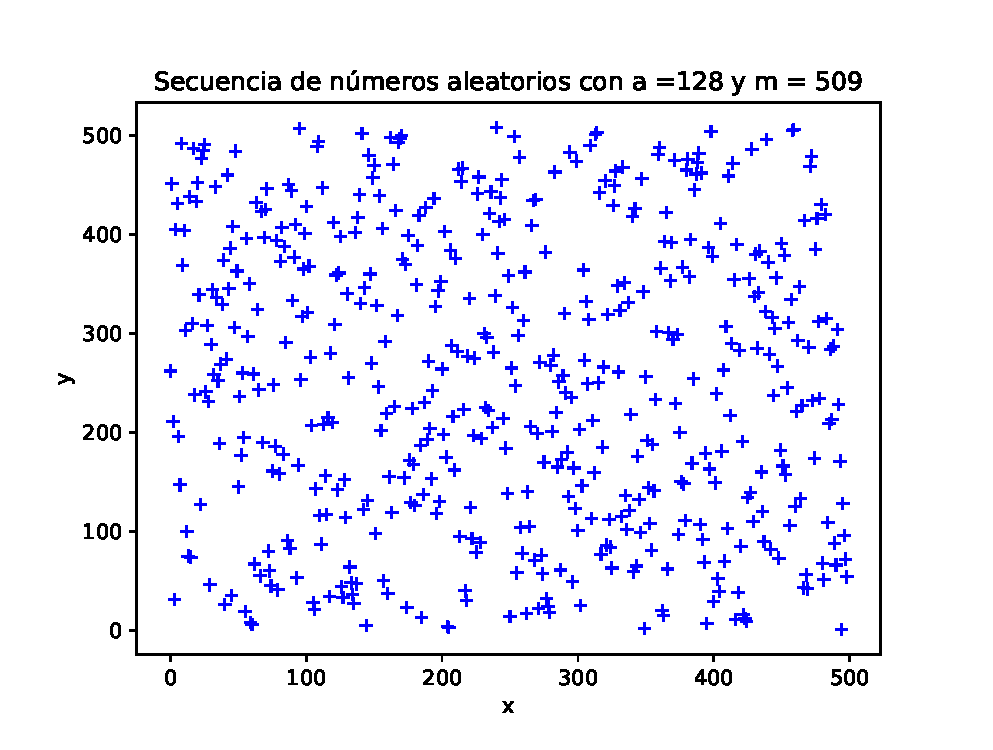
\includegraphics[scale=0.6]{Imagenes/Secuencia_aleatoria_01.eps}
\end{figure}
\end{frame}
\begin{frame}[fragile]
\frametitle{Distribución de números aleatorios (2/2)}
\begin{figure}
 \centering
 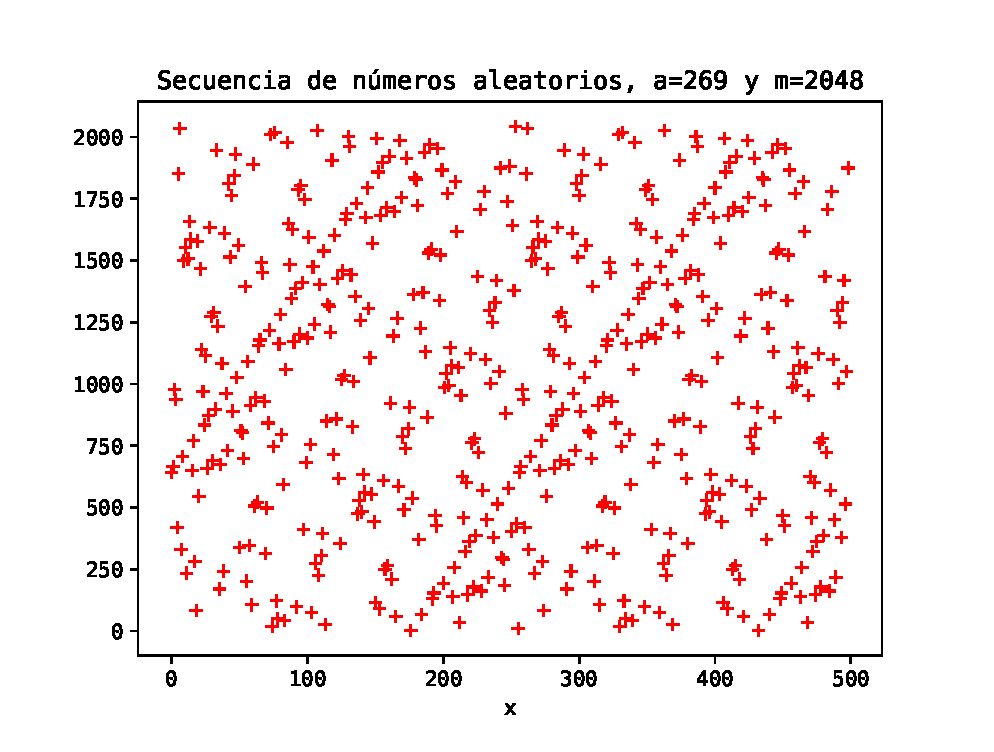
\includegraphics[scale=0.6]{Imagenes/Secuencia_aleatoria_02.eps}
\end{figure}
\end{frame}
\begin{frame}
\frametitle{Pregunta}
De las dos gráficas obtenidas: ¿Darías por hecho que las secuencias son aleatorios? ¿Hay algún patrón en la distribución de puntos?
\end{frame}
\subsection{La librería \texttt{random}}
\begin{frame}
\frametitle{La librería \texttt{random}}
Este módulo implementa generadores de números pseudoaleatorios para diversas distribuciones.
\\
\bigskip
Para números enteros, hay selección uniforme de un rango. Para las secuencias, hay una selección uniforme de un elemento aleatorio, una función para generar una permutación aleatoria de una lista \emph{in situ} y una función para el muestreo aleatorio sin reemplazo.
\end{frame}
\begin{frame}
\frametitle{La librería \texttt{random}}
Casi todas las funciones de la librería dependen de la función básica \funcionazul{random ()}, que genera un número flotante aleatorio de manera uniforme en el rango semiabierto $[0.0, 1.0)$
\end{frame}
\begin{frame}
\frametitle{La librería \texttt{random}}
En \python{} se usa el algoritmo \textoazul{Mersenne Twister} como generador central.
\\
\bigskip
Genera números flotantes de precisión de $53$ bits y tiene un período de $2^{19937}-1$.
\end{frame}
\begin{frame}
\frametitle{Alcance del generador en \texttt{random}}
El algoritmo \textoazul{Mersenne Twister} es uno de los generadores de números aleatorios más probados que existen.
\\
\bigskip
Sin embargo, al ser completamente determinista, no es adecuado para todos los propósitos, y es completamente inadecuado para fines criptográficos.
\end{frame}
\begin{frame}
\frametitle{Funciones importantes}
Dentro de la librería \funcionazul{random} existen distintas funciones que podremos utilizar, basta con revisar la documentación disponible, para identificar los parámetros y la respuesta que devuelve.
\end{frame}
\begin{frame}
\frametitle{Funciones importantes}
Mencionaremos dos funciones:
\setbeamercolor{item projected}{bg=green!70!black,fg=white}
\setbeamertemplate{enumerate items}[circle]
\begin{enumerate}[<+->]
\item \funcionazul{random.seed(a=None)}. Inicializa el generador de números aleatorios. Si no se especifica el valor de $a$, se utiliza el reloj del sistema. En caso de que $a$ sea un entero, se utiliza directamente.
\item \funcionazul{random.random()}. Devuelve un número de punto flotante en el rango $[0.0, 1.0)$.
\end{enumerate}
\end{frame}
\begin{frame}
\frametitle{Usando \texttt{seed} y \texttt{random}}
En el siguiente ejemplo se ejecuta el código para generar una secuencia de números aleatorios con la función \funcionazul{random}, que toma la semilla de la función \funcionazul{seed}.
\\
\bigskip
Al cerrar la ventana de la gráfica, se vuelve a ejecutar el código y veremos que la secuencia de números ya es distinta, debido a que se modificó la hora del sistema.
\end{frame}
\begin{frame}[allowframebreaks, fragile]
\frametitle{Ejemplo con \texttt{seed} y \texttt{random}}
\begin{lstlisting}[caption=Ejemplo de uso de las funciones del módulo \texttt{random}, style=codigopython]
import random

def generaazar(muestra, semilla=None):
    def arreglo(lista):
        for i in range(muestra):
            nuevoValor = random.random()
            lista.append(nuevoValor)
        return lista
    
    random.seed(semilla)    
    listaA_1_B = []
    listaA_2_B = []
    valoresRandomX = arreglo(listaA_1_B)
    valoresRandomY = arreglo(listaA_2_B)
    return valoresRandomX, valoresRandomY

muestra = 500
xA_1_B, yA_1_B = generaazar(muestra)
\end{lstlisting}
\end{frame}
\begin{frame}
\frametitle{Gráficas obtenidas 1/2}
\begin{figure}[h!]
  \centering
  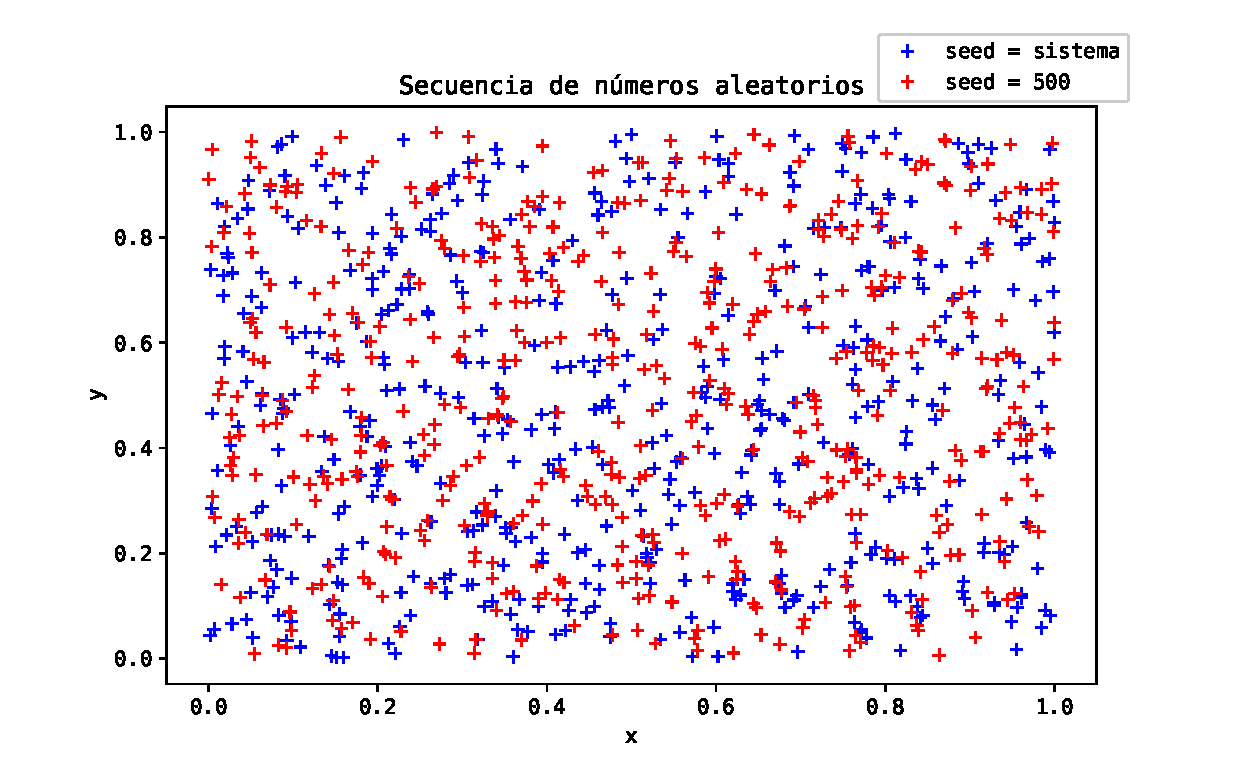
\includegraphics[scale=0.5]{Imagenes/Secuencia_aleatoria_03.eps}
\end{figure}
\end{frame}
\begin{frame}
\frametitle{Gráficas obtenidas 2/2}
\begin{figure}[h!]
  \centering
  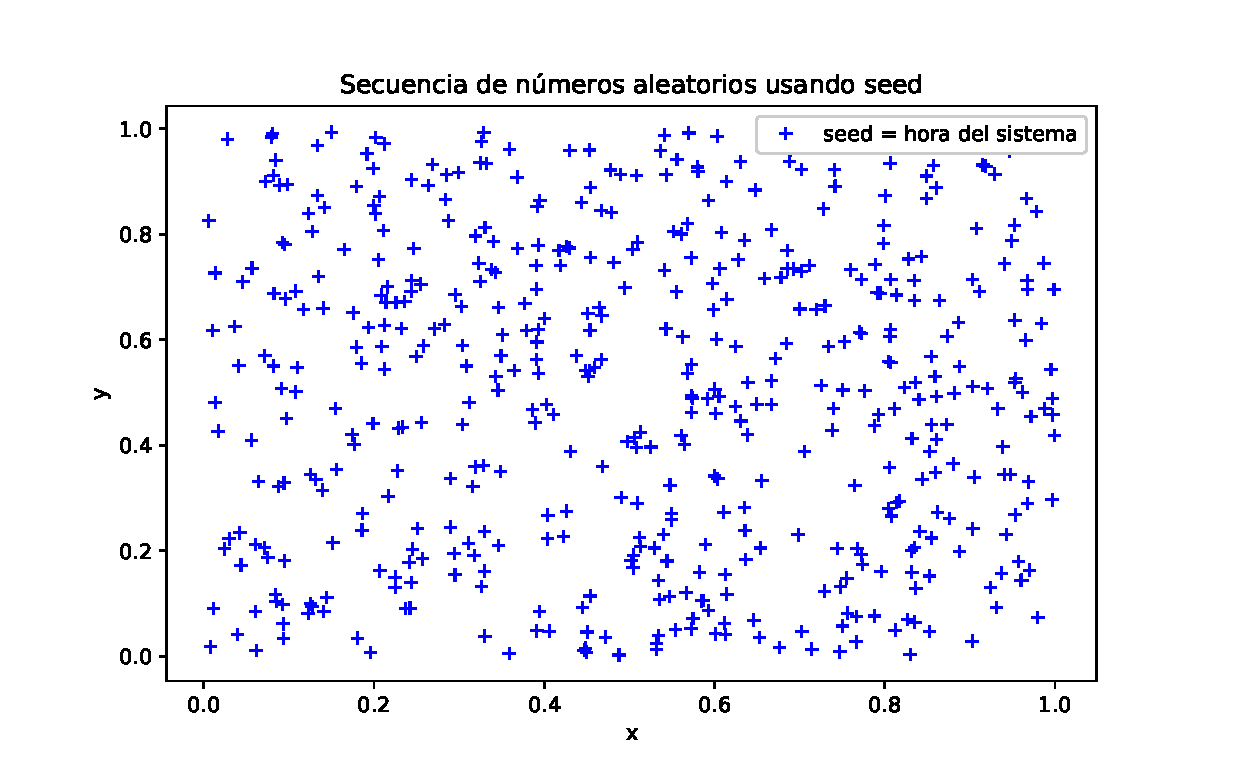
\includegraphics[scale=0.5]{Imagenes/Secuencia_aleatoria_04.eps}
\end{figure}
\end{frame}
\begin{frame}
\frametitle{Sobre las gráficas}
Las gráficas anteriores se obtuvieron con el mismo código, habiendo un cambio en el reloj del equipo, entonces la distribución de números aleatorios se modifica.
\end{frame}
\begin{frame}
\frametitle{Ejemplo con \texttt{random.seed(a)}}
Haremos un ejercicio en donde se van a generar dos secuencias de números con la función \funcionazul{random.seed(a)}, cambiaremos el valor de la semilla y vamos a comparar los resultados en una gráfica.
\\
\bigskip
Vamos a agregar una línea de código, la rutina de graficación habrá que implementarla.
\end{frame}
\begin{frame}[plain, allowframebreaks, fragile]
\frametitle{Código usando \texttt{seed()}}
\begin{lstlisting}[caption=Código con números generados con la hora del sistema y con semillas, style=codigopython]
xA_2_B, yA_2_B = generaazar(muestra, 500)
\end{lstlisting}
\end{frame}
\begin{frame}[fragile]
\frametitle{Gráfica obtenida}
\begin{figure}
 \centering
 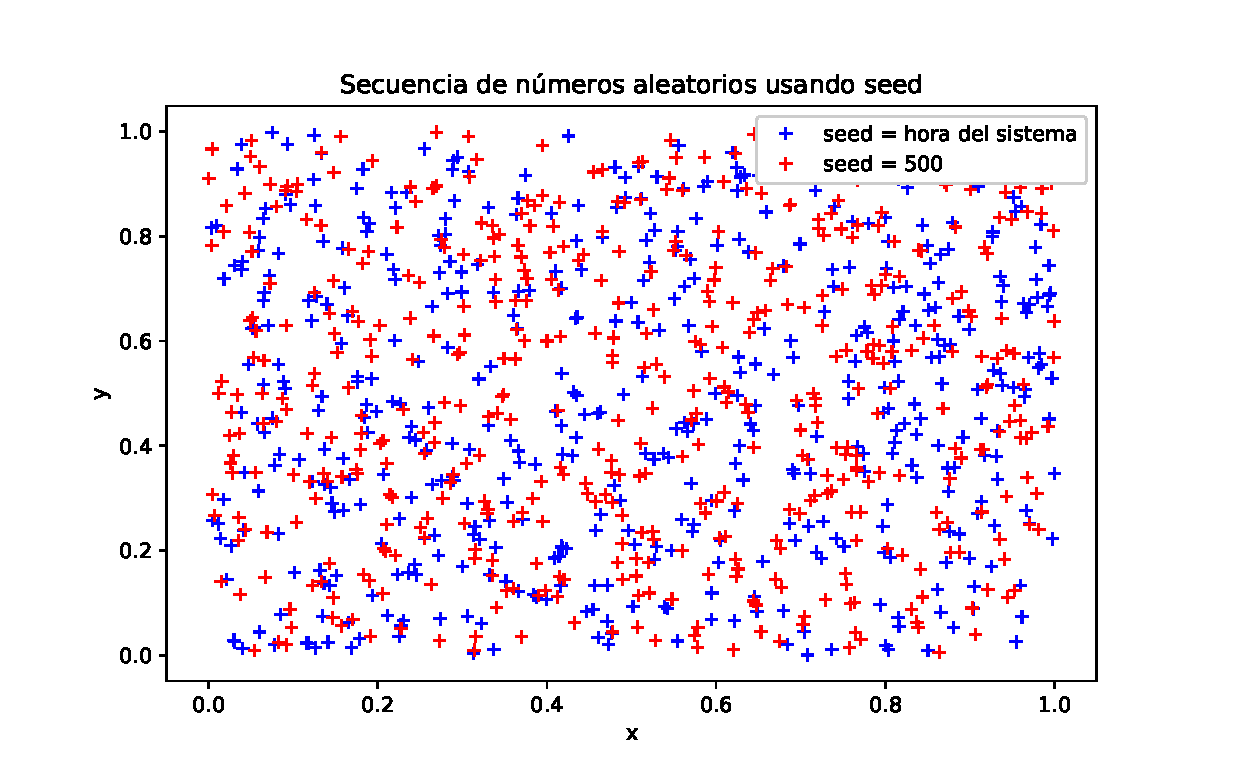
\includegraphics[scale=0.5]{Imagenes/Secuencia_aleatoria_05.eps}
\end{figure}
\end{frame}
\section{La aguja de Buffon}
\frame{\tableofcontents[currentsection, hideothersubsections]}
\subsection{Planteamiento}
\begin{frame}
\frametitle{La aguja de Buffon}
Resulta que $\pi$ también desempeña un papel importante en un experimento llamado \enquote{el problema de la aguja de Buffon}.
\\
\bigskip
\pause
El cual determina la probabilidad de que una aguja de longitud $\ell$, arrojada aleatoriamente aterrice en medio o atravesando una serie de líneas paralelas en el suelo.
\end{frame}
\begin{frame}
\begin{figure}
	\centering
	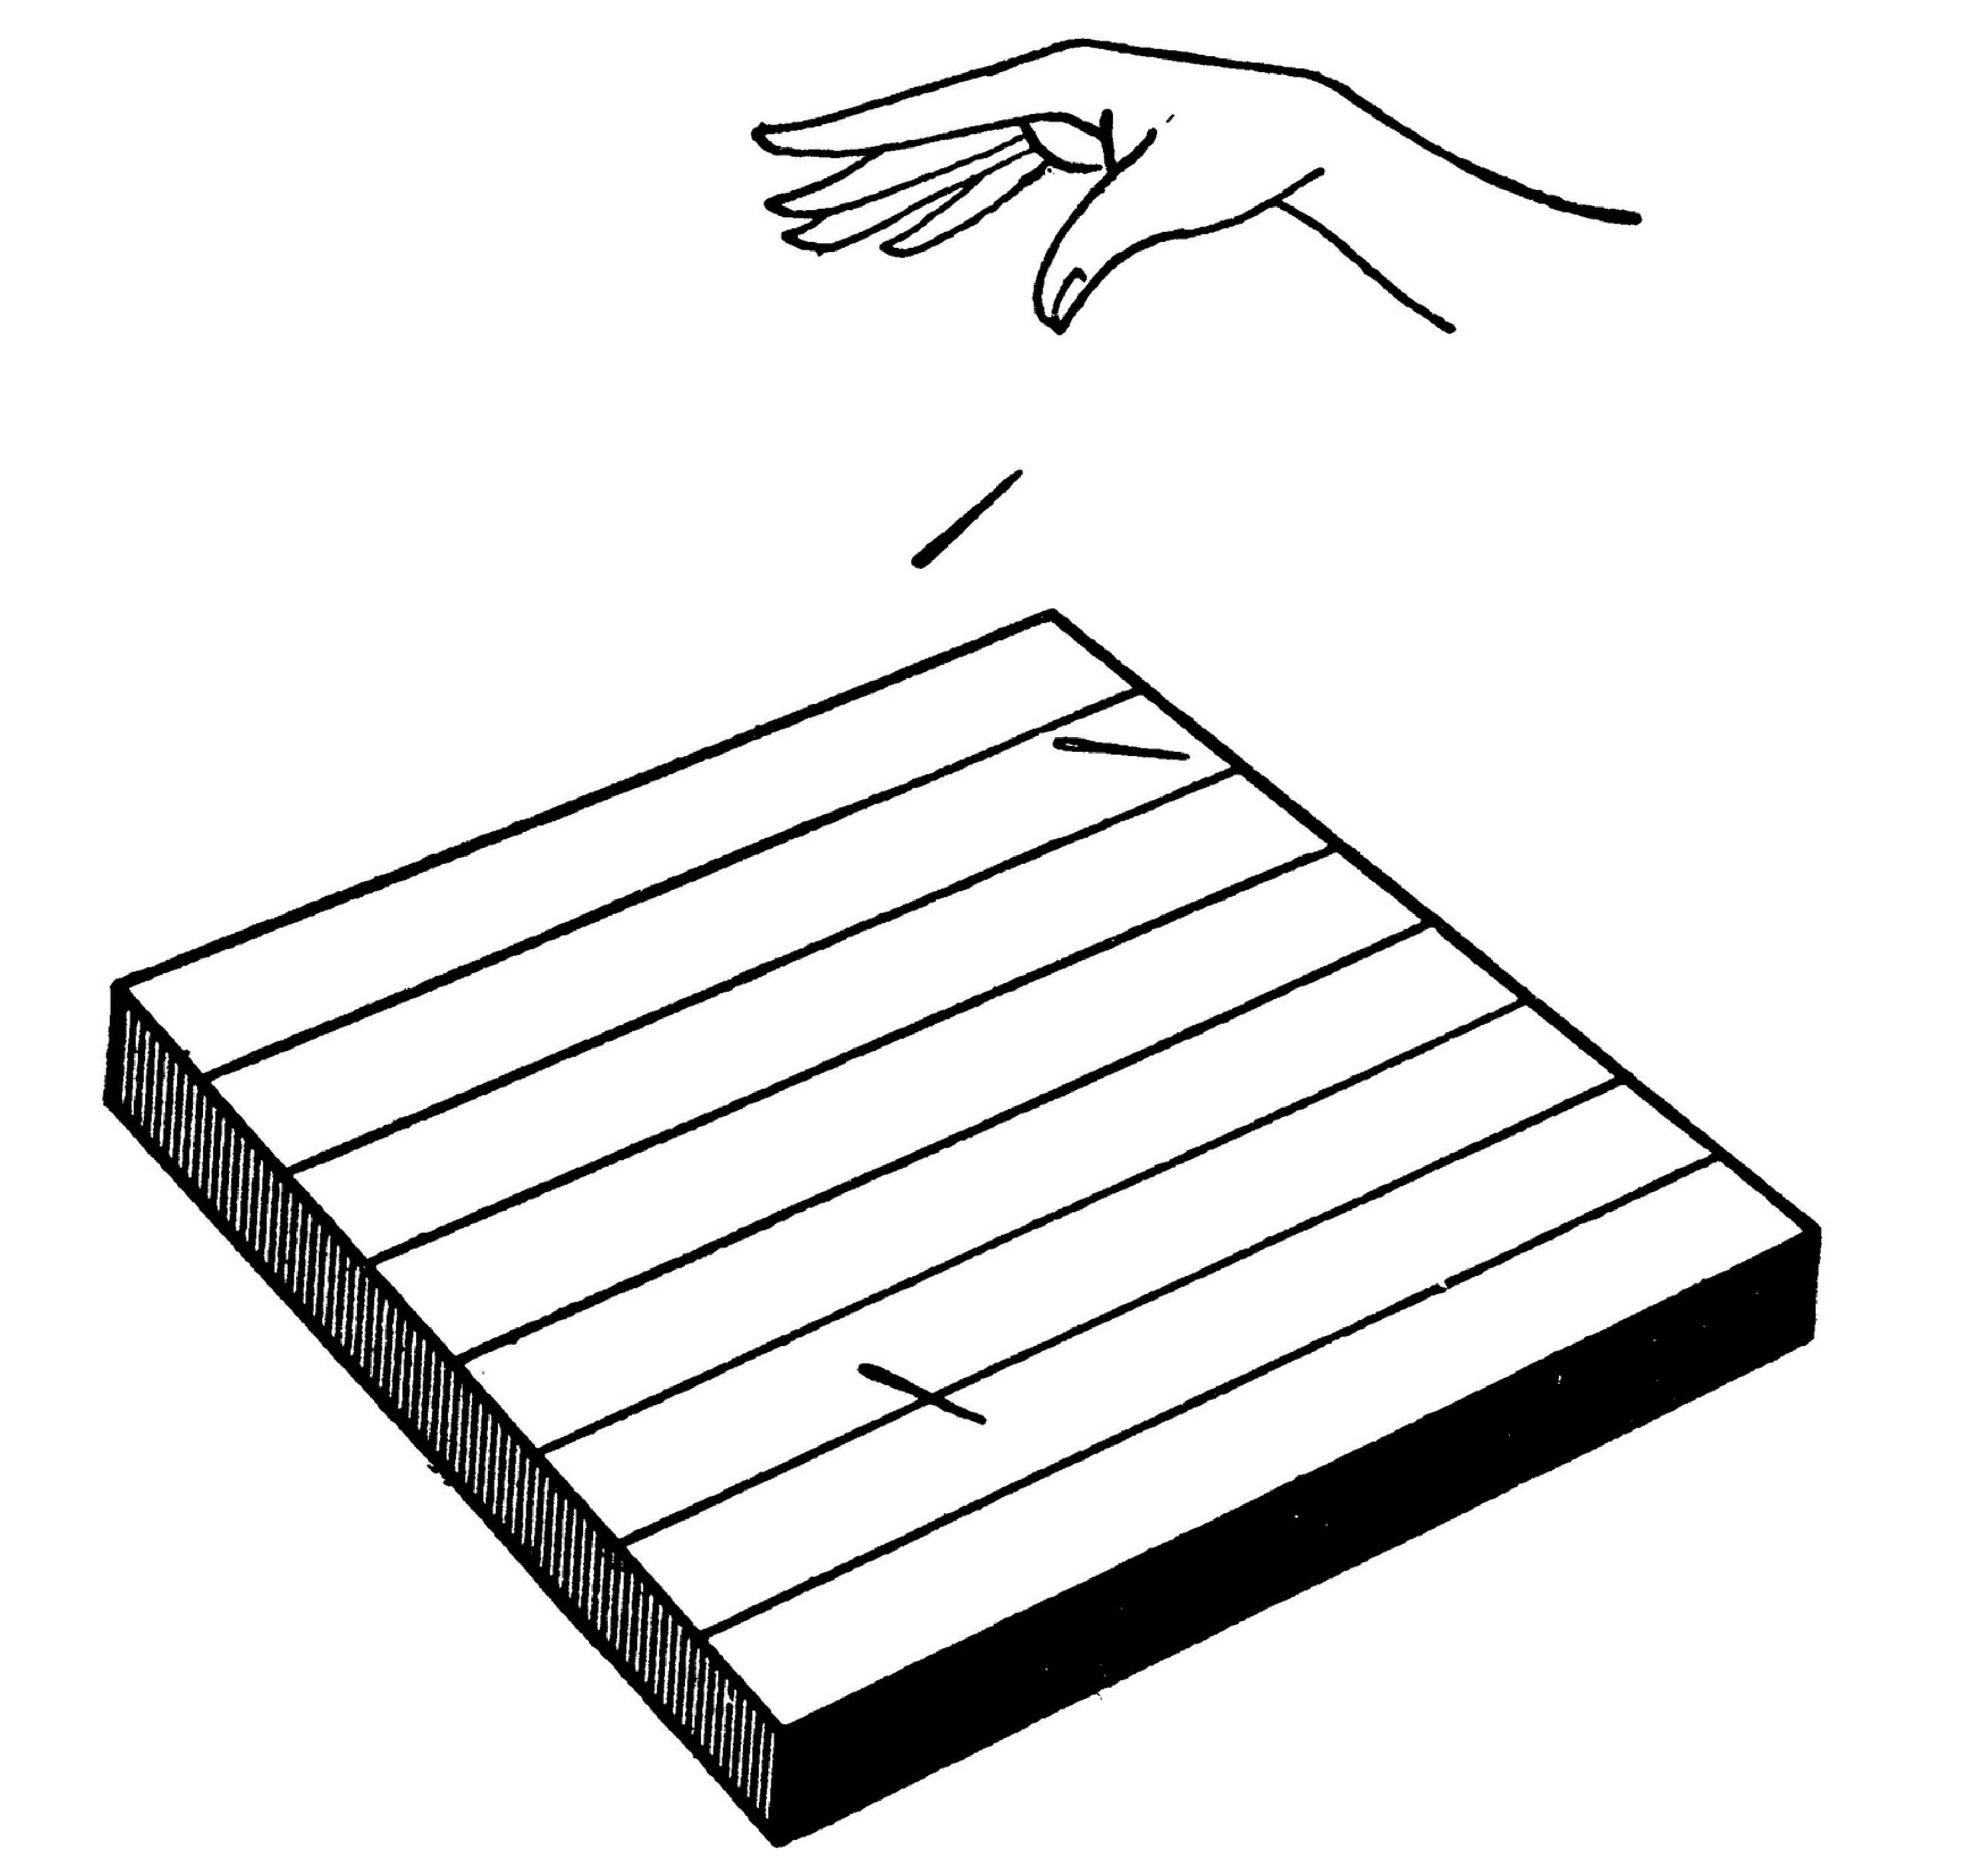
\includegraphics[scale=0.10]{Imagenes/aguja-de-buffon.eps}
\end{figure}
La separación entre las líneas es constante.
\end{frame}
\begin{frame}
\frametitle{La aguja de Buffon}
Resulta que si la distancia entre las líneas paralelas es la misma que la longitud $\ell$ de la aguja lanzada, el número de veces que la aguja cae atravesando las líneas (luego de un gran número de lanzamientos), nos servirá para calcular el valor de $\pi$.
\end{frame}
\subsection{Aproximación al valor de $\pi$}
\begin{frame}
\frametitle{Aproximación al valor de $\pi$}
De esa manera: 
\begin{align*}
\pi = \dfrac {2 \, N}{A}
\end{align*}
siendo $N$ el número total de intentos y $A$ el número de veces que la aguja ha cruzado alguna línea.
\end{frame}
\begin{frame}
\frametitle{Primer problema de tarea}
Considera el caso en el que la longitud de la aguja es igual a la separación entre las rayas, es decir $\ell = h$.
\\
\bigskip
Si la aguja cruza una línea de manera oblicua, es decir, existe un ángulo de inclinación con respecto a la línea, puedes deducir la relación a partir de la \enquote{función} que describe el caso de las agujas que tocan las líneas.
\end{frame}
% \begin{frame}
% \frametitle{Segundo problema de tarea}
% Una vez que has deducido el problema, implementa en python un programa que calcule el valor aproximado de $\pi$, a partir del número de lanzamientos, y el número de agujas que cruzan una línea.
% \\
% \bigskip
% En las siguientes gráficas verás los resultados cuando se realiza el lanzamiento de $10^{2}, 10^{3}, 10^{4}, 10^{5}, 10^{6}$ agujas.
% \end{frame}
% % \begin{frame}
% % \frametitle{Configuración para el problema de la aguja}
% % \begin{figure}[fragile]
% % \begin{tikzpicture}{font=\small}
% % 	\draw [thick] (0, 0) -- (7,0);
% % 	\draw [thick] (0, 4) -- (7,4);
% % 	\draw [<->] (1,0) -- node[left] {Distancia entre líneas = 1}(1, 4);
% % \end{tikzpicture}
% % \end{figure}
% % \end{frame}
% \begin{frame}
% \frametitle{Solución con python}
% \begin{figure}
%  \centering
%  \includegraphics[scale=0.6]{aproximacionPi_100.eps}
% \end{figure}
% \end{frame}
% \begin{frame}
% \frametitle{Solución con python}
% \begin{figure}
%  \centering
%  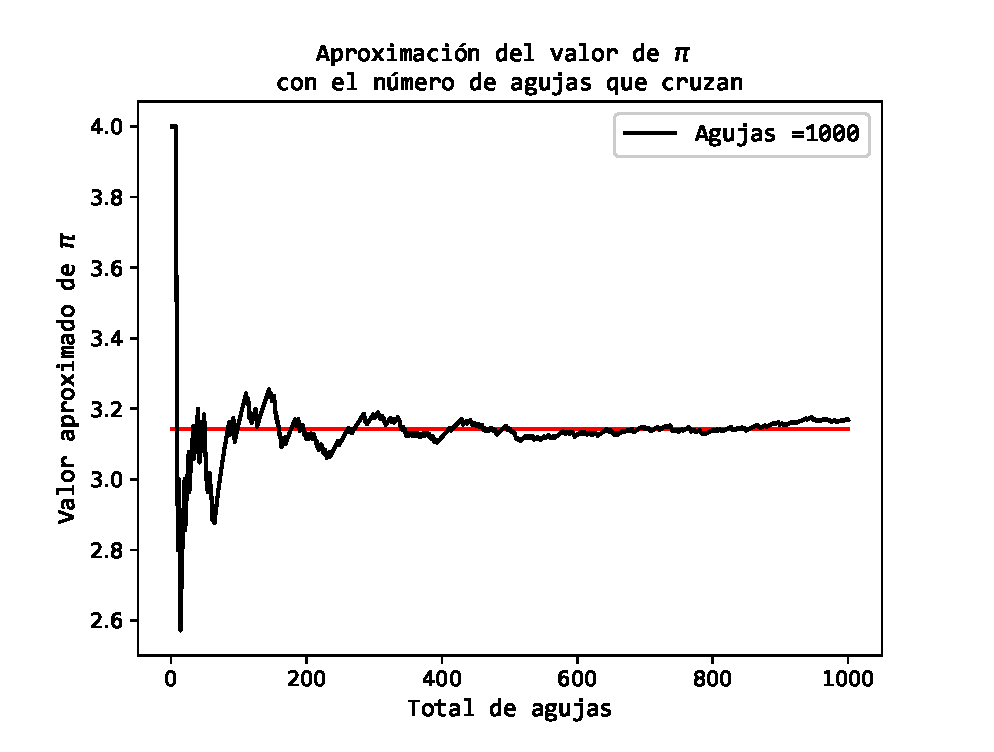
\includegraphics[scale=0.6]{aproximacionPi_1000.eps}
% \end{figure}
% \end{frame}
% \begin{frame}
% \frametitle{Solución con python}
% \begin{figure}
%  \centering
%  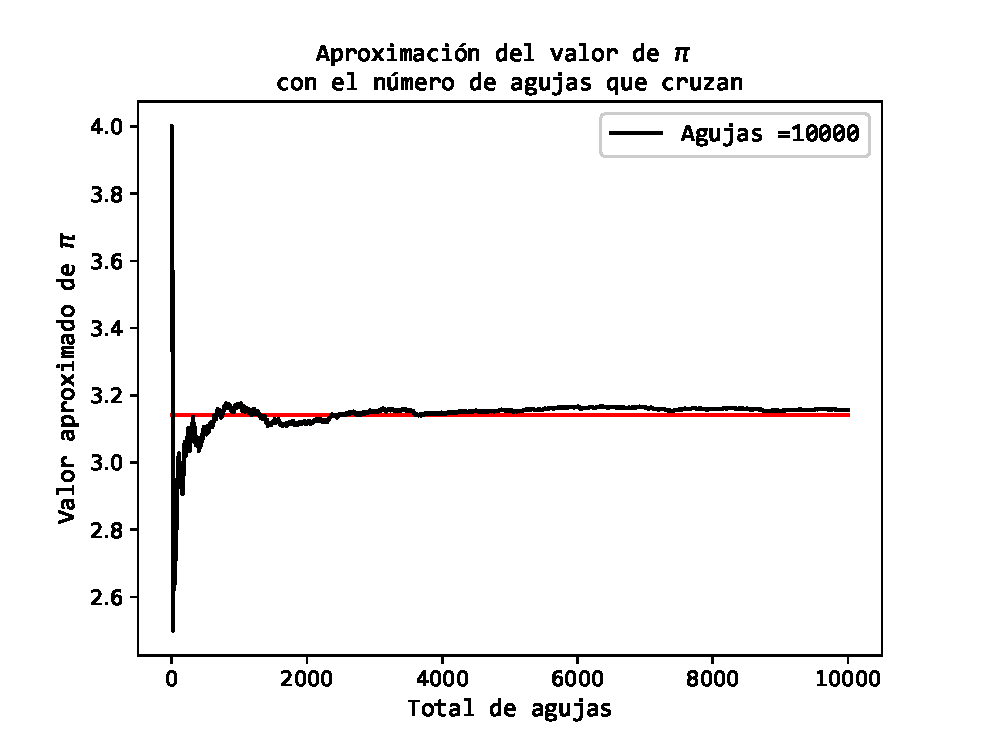
\includegraphics[scale=0.6]{aproximacionPi_10000.eps}
% \end{figure}
% \end{frame}
% \begin{frame}
% \frametitle{Solución con python}
% \begin{figure}
%  \centering
%  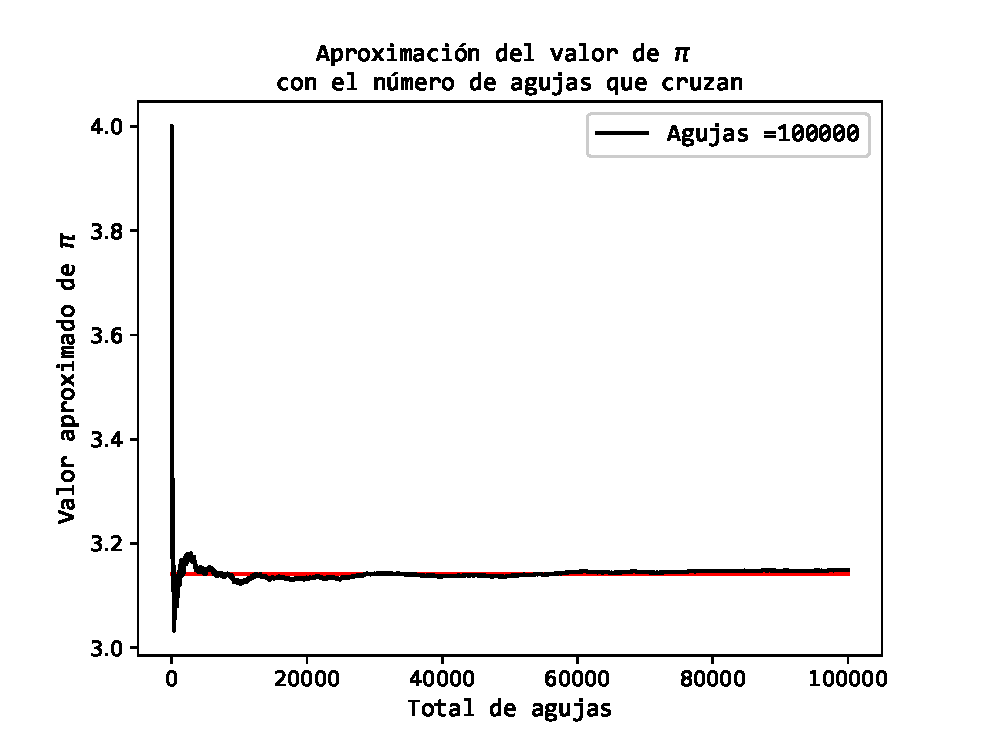
\includegraphics[scale=0.6]{aproximacionPi_100000.eps}
% \end{figure}
% \end{frame}
% \begin{frame}
% \frametitle{Solución con python}
% \begin{figure}
%  \centering
%  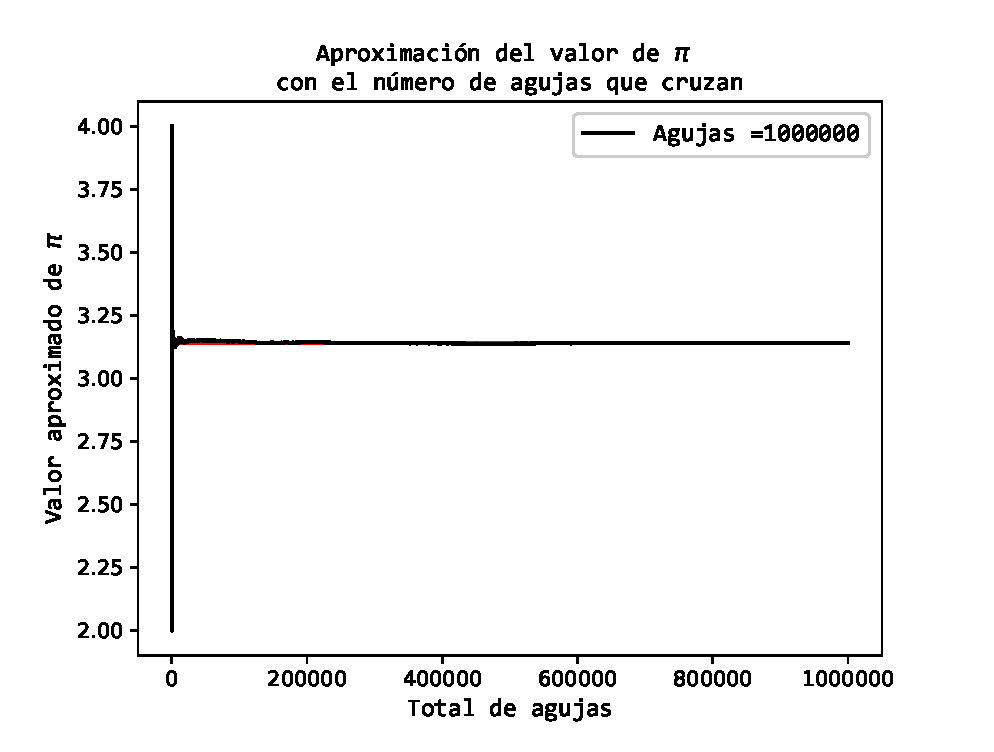
\includegraphics[scale=0.6]{aproximacionPi_1000000.eps}
% \end{figure}
% \end{frame}
\end{document}